\section{NET-08 BGP}


\subsection{Routing protocols e Autonomous Systems}

\subsubsection{Routing table, forwarding table e coesistenza di protocolli}

\paragraph{Obiettivo dei protocolli di routing e popolamento della routing table}

L’obiettivo dei protocolli di routing è costruire e mantenere automaticamente le \emph{routing table} dei router, secondo le policy amministrative configurate. Essi operano nel \emph{control plane}: scambiano informazioni di raggiungibilità, calcolano le rotte e aggiornano la \emph{routing table} logica.

Nel router è utile distinguere tra:
\begin{itemize}
    \item \textbf{routing table}: contiene tutte le rotte apprese (eventualmente più rotte per lo stesso prefisso);
    \item \textbf{forwarding table} o Forwarding Information Base (FIB): contiene le sole rotte selezionate come migliori, consultate dal \emph{data plane} per inoltrare i pacchetti.
\end{itemize}

Un algoritmo interno sceglie, per ogni prefisso, la \emph{best route} tra le rotte candidate presenti nella routing table e la inserisce nella FIB.

\paragraph{Presenza di più route per lo stesso prefisso e scelta della best route}

Nelle reti reali è normale che esistano più rotte verso lo stesso prefisso (ad esempio per ridondanza o multi-homing). Per un certo prefisso possono coesistere, sullo stesso router, rotte:
\begin{itemize}
    \item apprese da protocolli diversi (es. OSPF, BGP, route statica);
    \item apprese dallo stesso protocollo ma con next hop diversi.
\end{itemize}

La scelta della best route avviene in due fasi:
\begin{enumerate}
    \item \textbf{Confronto tra protocolli diversi}: si usa l'\emph{Administrative Distance (AD)} per stabilire quale protocollo sia più “credibile”.
    \item \textbf{Confronto all’interno dello stesso protocollo}: si usa la metrica specifica (hop count per RIP, costo di link per OSPF, AS path e altri attributi per BGP, ecc.).
\end{enumerate}

Ad esempio, in BGP, tra due annunci verso lo stesso prefisso con AS path di lunghezza diversa, viene in genere preferita la rotta con AS path più corto, che sarà installata nella routing table globale come best route BGP.

\subsubsection{IGP, EGP e modello ad Autonomous Systems}

\paragraph{Interior Gateway Protocols: Distance Vector (RIP) e Link-State (OSPF, IS-IS)}

Gli \emph{Interior Gateway Protocol (IGP)} operano all’interno di un singolo Autonomous System (AS) e calcolano le rotte \emph{intra-AS}. Esistono due principali famiglie:

\begin{itemize}
    \item \textbf{Distance Vector} (es. Routing Information Protocol, RIP): ogni router mantiene per ciascuna destinazione una distanza (tipicamente in hop) e scambia periodicamente la propria routing table con i vicini diretti. Il router non conosce la topologia completa, ma solo la distanza verso le destinazioni.
    \item \textbf{Link-State} (es. Open Shortest Path First, OSPF; Intermediate System to Intermediate System, IS-IS): i router diffondono informazioni sullo stato dei link (\emph{link-state advertisements}) e ogni nodo ricostruisce localmente la topologia dell’area, calcolando i cammini minimi (tipicamente con Dijkstra) verso tutte le destinazioni.
\end{itemize}

\paragraph{Exterior Gateway Protocols: ruolo di BGP tra AS diversi}

Gli \emph{Exterior Gateway Protocol (EGP)} scambiano informazioni di routing tra Autonomous Systems differenti, che corrispondono a domini amministrativi indipendenti (ISP o grandi organizzazioni). Il protocollo EGP di riferimento è Border Gateway Protocol versione 4 (BGP4).

BGP è un protocollo di tipo \emph{path-vector}: ogni annuncio di rotta contiene almeno:
\begin{itemize}
    \item il prefisso di rete;
    \item l’\emph{AS path}, cioè la sequenza di Autonomous Systems attraversati;
    \item il next hop.
\end{itemize}

La metrica di base è la lunghezza dell’AS path, integrata da altri attributi di routing e di policy. In questo modo, BGP consente a ciascun AS di applicare le proprie politiche di instradamento pur cooperando con gli altri domini.

\begin{figure}[H]
\centering
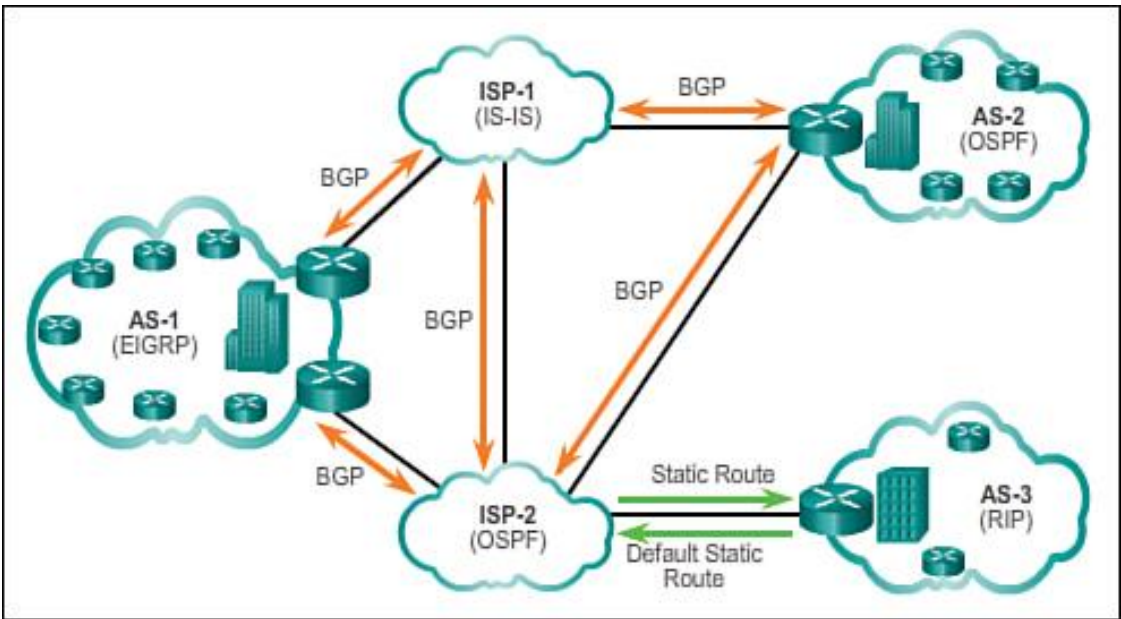
\includegraphics[width=0.75\textwidth]{immagini/NET_08/image_the_big_picture.png}
\caption{Visione d’insieme degli Autonomous Systems e del ruolo di BGP come protocollo EGP.}
\end{figure}

\paragraph{Concetto di Autonomous System, AS Number pubblico e privato}

Un \emph{Autonomous System (AS)} è un insieme di reti IP sotto il controllo amministrativo di una singola organizzazione, che applica una politica di routing coerente al proprio interno e verso l’esterno.

Ogni AS è identificato da un \emph{AS Number (ASN)}:
\begin{itemize}
    \item gli ASN “classici” a 16 bit sono compresi tra 1 e 65535;
    \item una parte di questo intervallo (64512–65535) è riservata ad ASN \emph{privati}, usati solo internamente e non visibili su Internet;
    \item con l’introduzione degli ASN a 32 bit è stato definito un ulteriore intervallo di ASN privati (ad esempio 4200000000–4294967294).
\end{itemize}

Gli ASN pubblici identificano univocamente l’AS nella rete globale e compaiono nei path BGP scambiati tra domini.

\subsubsection{Administrative Distance}

\paragraph{Definizione di AD e interazione tra protocolli di routing}

Quando su un router coesistono più protocolli di routing, è possibile che diversi protocolli forniscano rotte verso lo stesso prefisso. L’\emph{Administrative Distance (AD)} è il meccanismo con cui il router stabilisce quale protocollo sia più affidabile, prima ancora di confrontare le metriche interne.

L’AD ha le seguenti caratteristiche:
\begin{itemize}
    \item è un numero associato alle rotte apprese tramite un certo protocollo su quel router;
    \item valori più bassi indicano maggiore fiducia;
    \item è una proprietà \emph{locale}: non viene scambiata con altri router;
    \item entra in gioco solo quando più protocolli offrono rotte concorrenti per lo stesso prefisso; all’interno di un singolo protocollo si continua a usare la metrica specifica.
\end{itemize}

\paragraph{Valori tipici su IOS e impatto sulla scelta della route}

Su molte piattaforme (ad esempio Cisco IOS) si usano valori di AD di default che definiscono una gerarchia di fiducia tra le diverse fonti di routing, ad esempio:
\begin{itemize}
    \item \textbf{0}: rete \emph{directly connected};
    \item \textbf{1}: rotta \emph{statica};
    \item \textbf{20}: rotta appresa via External BGP (eBGP);
    \item circa \textbf{110}: rotta appresa via OSPF;
    \item \textbf{120}: rotta appresa via RIP;
    \item \textbf{200}: rotta appresa via Internal BGP (iBGP);
    \item \textbf{255}: rotta non utilizzabile (non viene mai scelta come best route).
\end{itemize}

Di conseguenza, se un router impara una rotta verso lo stesso prefisso sia da eBGP sia da OSPF, la rotta eBGP (AD 20) viene preferita a quella OSPF (AD 110). Una rotta statica (AD 1) ha priorità rispetto alle rotte dinamiche, a meno che l’operatore non modifichi esplicitamente i valori di AD. In questo modello, l’AD è il primo criterio di selezione tra protocolli diversi; la metrica interna al protocollo viene applicata solo tra rotte candidate con la stessa AD.
\begin{figure}[H]
\centering
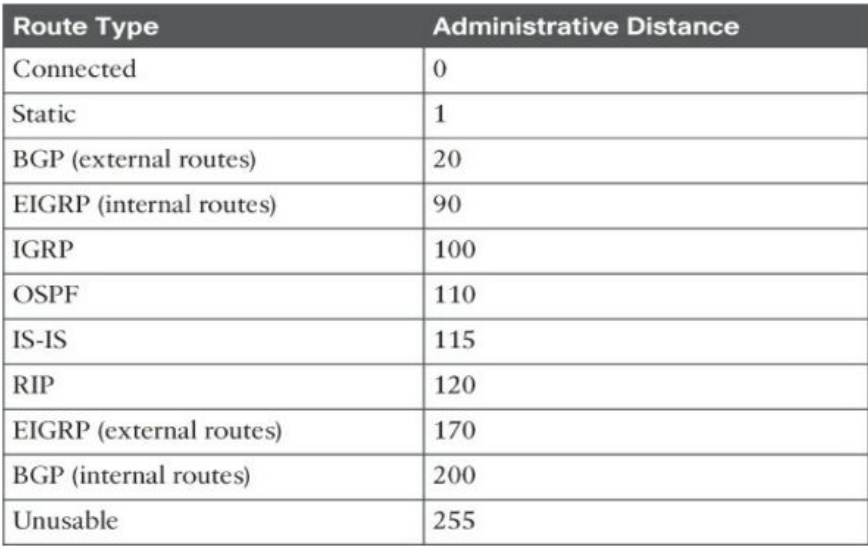
\includegraphics[width=0.75\textwidth]{immagini/NET_08/image_ad_cisco_ios.png}
\caption{Valori di default dell’Administrative Distance su Cisco IOS e priorità tra le diverse fonti di routing.}
\end{figure}

\subsection{Concetti di base di BGP}

\subsubsection{BGP come path-vector routing protocol}

\paragraph{Differenze rispetto a distance vector classici}

Border Gateway Protocol (BGP) è un protocollo di tipo \emph{path-vector}, derivato dal modello \emph{distance vector}. Come nei distance vector classici, un router BGP riceve rotte dai vicini, calcola localmente le proprie scelte di instradamento e annuncia i risultati agli altri peer. La differenza principale è che, invece di una semplice distanza numerica, BGP usa come metrica il vettore \texttt{AS\_PATH}, che descrive esplicitamente la sequenza di Autonomous Systems attraversati e permette di prendere decisioni basate sull’intero cammino logico, non solo su un costo aggregato.

\paragraph{AS\_PATH come descrizione del cammino tra AS}

Nel modello path-vector, ogni annuncio BGP (in uno scenario semplice) contiene almeno tre informazioni fondamentali: il prefisso di rete destinazione, il \emph{path vector} e il \emph{next hop}. Il path vector coincide con l’attributo \texttt{AS\_PATH} e rappresenta la lista ordinata degli Autonomous Systems attraversati per raggiungere la destinazione. Quando un annuncio BGP esce da un AS, il router di frontiera prepende a \texttt{AS\_PATH} il proprio AS Number, così che, man mano che la rotta si propaga, la lista degli AS visitati si arricchisce. In questo modo \texttt{AS\_PATH} descrive in maniera esplicita il cammino inter-AS e può essere utilizzato sia come metrica (preferendo, in prima approssimazione, il cammino con lista più corta), sia come base per politiche di instradamento più avanzate.

\paragraph{Autonomous System Numbers a 2 e 4 byte}

Ogni Autonomous System è identificato da un numero, l’\emph{Autonomous System Number (ASN)}. Storicamente gli ASN erano codificati su 16 bit, con valori compresi tra 1 e 65535. All’interno di questo intervallo è definita una sotto-classe di ASN \emph{privati}, tipicamente compresi tra 64512 e 65535, destinati a scenari che non richiedono visibilità globale. L’esaurimento dello spazio a 16 bit ha portato all’introduzione degli \emph{AS Number a 32 bit} (RFC 6793), che estendono il namespace e prevedono a loro volta un intervallo dedicato di ASN privati, ad esempio tra 4200000000 e 4294967294.

\subsubsection{Sessioni BGP e scambio di informazioni}

\paragraph{BGP su TCP porta 179: neighbors, BGP speaker}

BGP opera sopra TCP: prima che due router possano scambiarsi messaggi BGP, devono stabilire una connessione TCP attraverso il consueto \emph{three-way handshake}, utilizzando la porta ben nota 179 sul peer remoto. Una volta instaurata la sessione TCP, i due router sono detti \emph{neighbors} o \emph{peers}, mentre ciascun router che esegue BGP è chiamato \emph{BGP speaker}. Tutti i messaggi BGP vengono scambiati in unicast sulla connessione TCP tra due soli peer, che ne garantisce affidabilità e ordinamento.

\paragraph{Tipi di messaggi: OPEN, KEEPALIVE, UPDATE, NOTIFICATION}

Dopo l’apertura della connessione TCP, i peer BGP si scambiano messaggi per negoziare i parametri della sessione e diffondere le informazioni di routing. Il protocollo definisce quattro tipi di messaggi:
\begin{itemize}
    \item \textbf{OPEN}, usato per instaurare la sessione BGP e concordare i parametri di base (versione, ASN, timer, ecc.);
    \item \textbf{KEEPALIVE}, usato per mantenere viva la sessione e verificare la raggiungibilità del peer;
    \item \textbf{UPDATE}, che trasporta gli annunci di nuove rotte e le eventuali revoche di rotte non più valide;
    \item \textbf{NOTIFICATION}, usato per segnalare condizioni di errore e, in genere, chiudere la sessione BGP.
\end{itemize}

\paragraph{Scambio iniziale completo e aggiornamenti incrementali}

Quando due peer stabiliscono per la prima volta una sessione BGP, dopo l’handshake TCP e i messaggi di apertura, ciascuno invia all’altro l’intera propria BGP routing table, così da allineare completamente la vista delle rotte. Successivamente, lo scambio diventa \emph{incrementale}: i peer inviano solo UPDATE parziali contenenti le modifiche rispetto allo stato precedente (nuove rotte o ritiri di rotte esistenti). In parallelo vengono scambiati periodicamente messaggi KEEPALIVE; se un router non riceve KEEPALIVE per un certo numero di intervalli (ad esempio tre), dichiara il peer inattivo e rimuove dalla propria tabella tutte le rotte apprese tramite quel neighbor.

\subsubsection{Tabelle BGP e ruoli di IBGP/EBGP}

\paragraph{BGP table vs IP routing table}

I router che eseguono BGP mantengono una struttura dati specifica, la \emph{BGP table}, distinta dalla IP routing table. Nella BGP table vengono memorizzate tutte le rotte apprese tramite UPDATE dai vari peer, insieme ai rispettivi attributi. Su queste rotte il router applica filtri e politiche (ad esempio basate su \texttt{AS\_PATH} o altri attributi) e seleziona, per ciascun prefisso, un unico cammino considerato \emph{best path}. Solo le best route BGP diventano candidate a essere inserite nella IP routing table, dove competono con eventuali rotte provenienti da altri protocolli di routing o da configurazioni statiche.
\begin{figure}[H]
\centering
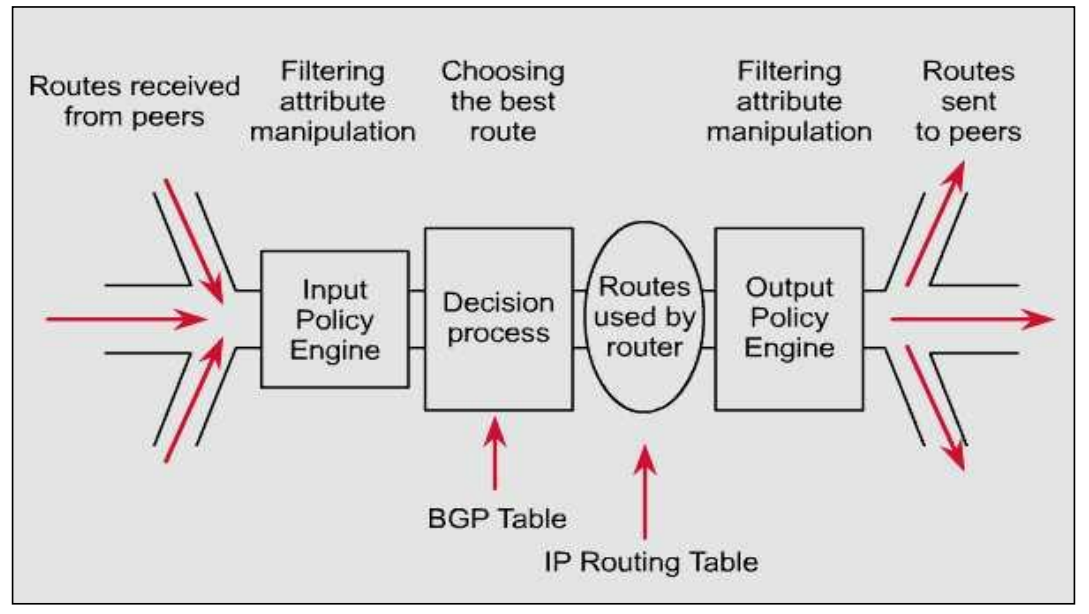
\includegraphics[width=0.75\textwidth]{immagini/NET_08/image_bgp_processing_pipeline.png}
\caption{Pipeline di elaborazione di BGP tra ricezione degli UPDATE, tabella BGP, scelta del best path e aggiornamento della routing table IP.}
\end{figure}

\paragraph{External BGP (EBGP) tra AS e border router}

Quando BGP è eseguito tra router appartenenti a Autonomous Systems differenti, si parla di \emph{External BGP} (EBGP). In questo caso i router che si trovano al confine dell’AS e instaurano sessioni EBGP con i router dell’Internet Service Provider o di altri AS sono detti \emph{border router}. Tramite EBGP, gli AS si scambiano le informazioni di raggiungibilità verso le rispettive reti pubbliche, applicando le proprie politiche di instradamento e di sicurezza.

\paragraph{Internal BGP (IBGP) all’interno dell’AS e transit router}

BGP non è limitato allo scambio di rotte tra AS diversi: può essere usato anche all’interno di un singolo AS per distribuire ai router interni le rotte verso destinazioni esterne. In questo caso si parla di \emph{Internal BGP} (IBGP). I router che eseguono IBGP e che si occupano di inoltrare il traffico tra peer interni sono spesso chiamati \emph{transit router}. IBGP consente agli apparati interni all’AS di avere una vista coerente delle rotte apprese tramite EBGP ai bordi della rete, supportando in particolare scenari di multi-homing e interconnessioni complesse.
\begin{figure}[H]
\centering
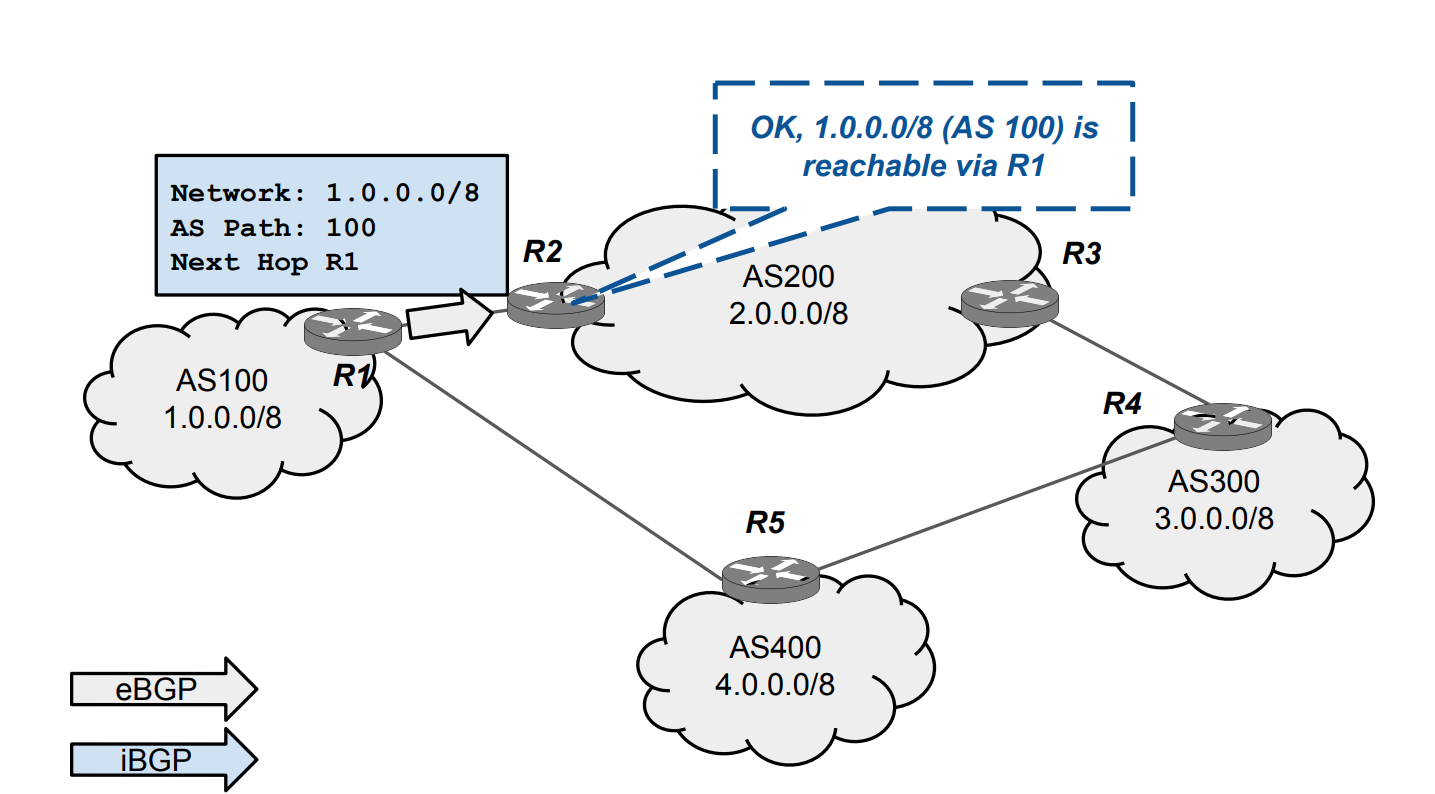
\includegraphics[width=0.75\textwidth]{immagini/NET_08/image_aspath_example.png}
\caption{Esempio di propagazione BGP del prefisso 1.0.0.0/8 tra più Autonomous Systems (AS\_PATH iniziale).}
\end{figure}

\subsubsection{Propagazione delle route e prevenzione dei loop}

\paragraph{Costruzione dell’AS\_PATH e scelta del cammino più corto}

Come visto in precedenza, quando una rotta viene propagata tramite BGP ogni AS prepende il proprio AS Number all’attributo \texttt{AS\_PATH}, così che la sequenza di AS rifletta il cammino inter-dominio seguito dall’annuncio. Se un router riceve più annunci per lo stesso prefisso con \texttt{AS\_PATH} diversi, può confrontarne la lunghezza: in scenari semplici viene preferita la rotta con \texttt{AS\_PATH} più corto, ossia quella che attraversa il minor numero di Autonomous Systems (ad esempio \texttt{100} rispetto a \texttt{100,200,300}), che sarà installata come best route nella IP routing table.
\begin{figure}[H]
\centering
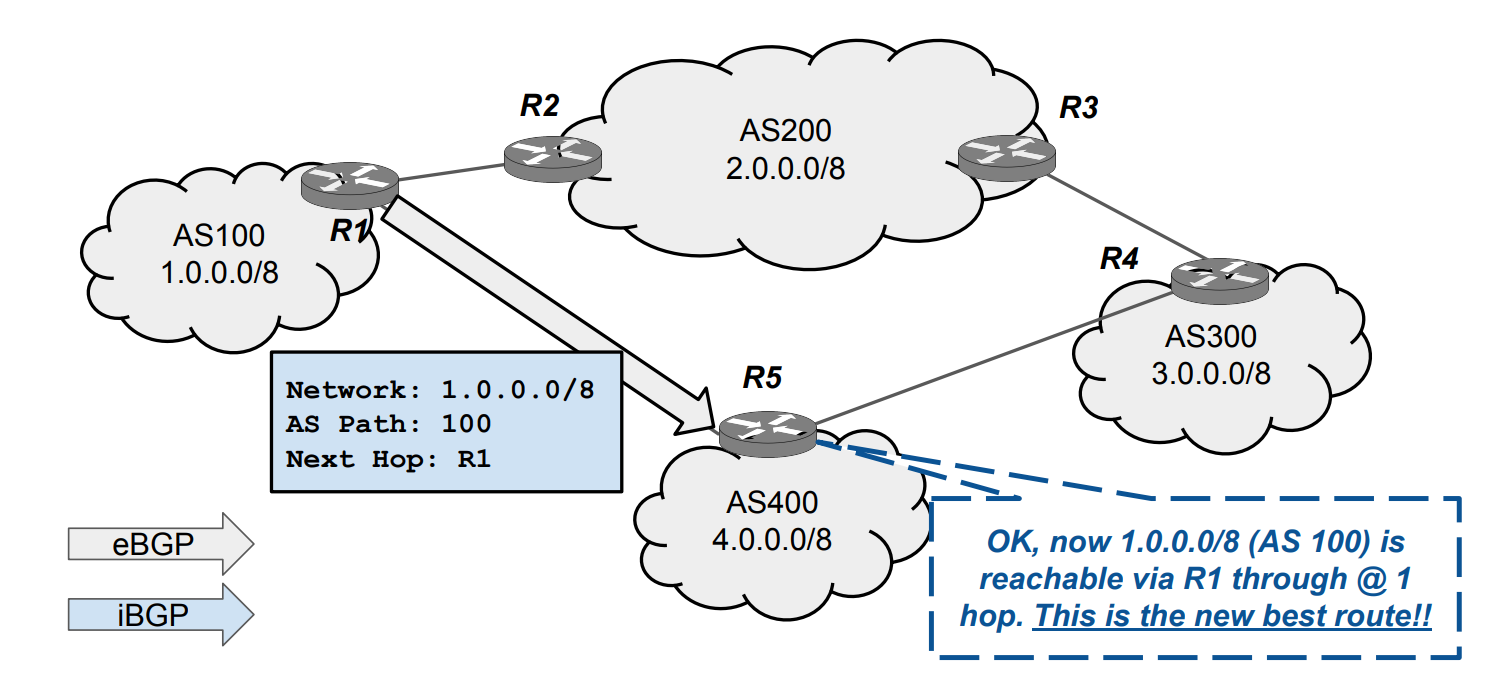
\includegraphics[width=0.75\textwidth]{immagini/NET_08/image_aspath_shortest_path.png}
\caption{Scelta del best path BGP verso 1.0.0.0/8 in base alla lunghezza dell’AS\_PATH.}
\end{figure}

\paragraph{Rilevamento dei loop tramite AS\_PATH}

La modalità di costruzione di \texttt{AS\_PATH} permette di rilevare facilmente eventuali loop inter-AS. Poiché un AS aggiunge il proprio numero solo quando un UPDATE esce dal dominio, un annuncio che rientri in un AS già presente nella lista presenterà necessariamente quell’ASN ripetuto all’interno di \texttt{AS\_PATH}. Un BGP speaker può quindi controllare se il proprio AS Number compare nella sequenza: in caso affermativo, l’annuncio viene scartato, evitando la formazione di cicli di instradamento tra domini diversi. Questo meccanismo di controllo sui path vector integra la semplice metrica numerica e costituisce una delle principali differenze rispetto ai distance vector classici.
\begin{figure}[H]
\centering
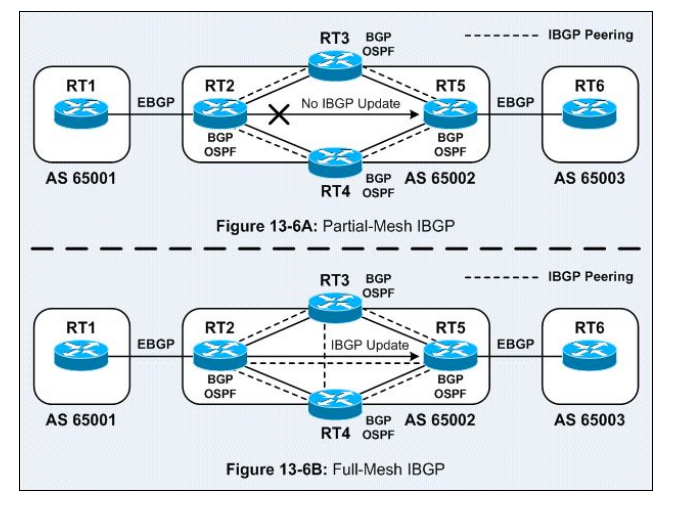
\includegraphics[width=0.75\textwidth]{immagini/NET_08/image_bgp_loop_avoidance.png}
\caption{Meccanismi di BGP per evitare loop tra AS (AS\_PATH) e all’interno di un AS (regola di Split Horizon).}
\end{figure}

\paragraph{Split Horizon IBGP, full-mesh e cenni ai Route Reflector}

Il controllo dei loop all’interno di un singolo AS non può basarsi su \texttt{AS\_PATH}, perché all’interno del dominio l’ASN è lo stesso per tutti i router. Per prevenire loop interni, BGP adotta una regola di \emph{Split Horizon} specifica:
\begin{itemize}
    \item una rotta appresa tramite IBGP non viene mai riannunciata ad altri peer IBGP;
    \item una rotta non viene mai pubblicizzata indietro allo stesso peer EBGP da cui è stata ricevuta.
\end{itemize}
Queste regole evitano la circolazione indefinita degli annunci dentro l’AS, ma hanno una conseguenza importante: se si vuole che tutti i router interni dispongano della vista completa delle rotte BGP, occorre creare una \emph{full-mesh} di sessioni IBGP tra tutti i BGP speaker interni. Per migliorare la scalabilità e ridurre il numero di sessioni necessarie, le implementazioni BGP introducono i \emph{Route Reflector}, nodi specializzati che riflettono selettivamente le rotte ai peer IBGP, limitando la necessità di connessioni dirette tra tutte le coppie di router.

\subsection{Attributi BGP e selezione del percorso}

\subsubsection{Classi di attributi e attributi obbligatori}

\paragraph{Well-known vs optional; mandatory vs discretionary}

Gli \emph{attributi BGP} fanno parte dei messaggi UPDATE e descrivono le caratteristiche di ciascun prefisso (informazioni di path, preferenza di rotta, next hop, dati di aggregazione, ecc.).

Le slide classificano gli attributi in quattro categorie principali:
\begin{itemize}
    \item \textbf{Well-known mandatory}: devono essere sempre presenti in ogni annuncio BGP e devono essere riconosciuti da ogni implementazione;
    \item \textbf{Well-known discretionary}: sono riconosciuti universalmente, ma la loro presenza in un annuncio è opzionale;
    \item \textbf{Optional transitive}: non sono necessariamente supportati da tutti i router, ma se un router non li riconosce deve comunque propagarli;
    \item \textbf{Optional non-transitive}: possono essere ignorati dai router che non li riconoscono e non sono propagati oltre quel nodo.
\end{itemize}

Non tutte le implementazioni supportano lo stesso insieme di attributi, ma le classi well-known garantiscono un nucleo comune di funzionalità.

\paragraph{Attributi chiave: DESTINATION, AS\_PATH, NEXT\_HOP}

Tre attributi sono indicati nelle slide come \emph{obbligatori} (well-known mandatory) per ogni rotta BGP:
\begin{itemize}
    \item \textbf{DESTINATION} (destination network): identifica il prefisso di rete annunciato;
    \item \textbf{AS\_PATH}: contiene la sequenza di Autonomous Systems attraversati per raggiungere il prefisso;
    \item \textbf{NEXT\_HOP}: specifica l’indirizzo IP del router a cui inoltrare il traffico per raggiungere la destinazione.
\end{itemize}

Questi tre attributi costituiscono il nucleo minimo di informazione per descrivere una rotta BGP: cosa si raggiunge (DESTINATION), attraverso quali AS (AS\_PATH) e tramite quale prossimo hop (NEXT\_HOP).

\subsubsection{Criteri di selezione del best path}

\paragraph{Ordine generale di decisione (Weight, Local Pref, AS\_PATH, MED, ecc.)}

BGP seleziona un solo \emph{best path} per ogni destinazione. Una volta scelto, il percorso viene inserito nella BGP routing table e può essere propagato ai neighbor. L’AS\_PATH è solo uno dei criteri: le slide riportano una sequenza di decisione (dipendente in parte dall’implementazione) riassunta dal mnemonico “\emph{We Love Oranges AS Oranges Mean Pure Refreshment}”:
\begin{enumerate}
    \item \textbf{Weight} (W): valore locale, specifico del router (tipicamente proprietario del vendor); si preferisce il percorso con weight più alto;
    \item \textbf{LOCAL\_PREF} (L): preferenza locale distribuita all’interno dell’AS; si preferisce il valore più alto;
    \item \textbf{Originate} (O): sono preferite le rotte originate localmente rispetto a quelle apprese da altri peer;
    \item \textbf{AS\_PATH} (AS): tra più percorsi, si preferisce quello con AS\_PATH più corto;
    \item \textbf{ORIGIN code} (O): a parità di AS\_PATH, si preferiscono rotte con origine IGP rispetto a EGP, e queste rispetto a \emph{incomplete};
    \item \textbf{MED} (M): \emph{Multi-Exit Discriminator}; si preferisce il valore più basso;
    \item \textbf{Paths type} (P): a parità dei criteri precedenti, si preferiscono percorsi \emph{External} (EBGP) rispetto a \emph{Internal} (IBGP);
    \item \textbf{Router ID} (R): come tie-break finale, si sceglie il percorso proveniente dal router con ID più basso.
\end{enumerate}

Ogni attributo ha un significato operativo specifico e può essere usato per costruire politiche di instradamento personalizzate.

\paragraph{Preferenza per EBGP vs IBGP e tie-break finali}

Un punto sottolineato nella sequenza di selezione è la preferenza per i percorsi \emph{esterni} rispetto a quelli \emph{interni}: quando tutte le altre condizioni sono equivalenti, BGP tende a preferire una rotta appresa tramite EBGP rispetto a una rotta IBGP per lo stesso prefisso. Se anche questo criterio non distingue le rotte, il router utilizza il Router ID come tie-break finale, scegliendo l’annuncio proveniente dal BGP speaker con identificativo numericamente più piccolo.

\subsubsection{Manipolazione degli attributi}

\paragraph{Politiche in ingresso e in uscita (filtri e riscritture)}

Le slide evidenziano che gli attributi BGP possono essere \emph{manipolati} (modificati, aggiunti o rimossi) sia:
\begin{itemize}
    \item in \textbf{ingresso}, subito dopo la ricezione di UPDATE BGP, prima che il router esegua la selezione del best path;
    \item in \textbf{uscita}, prima di inviare UPDATE ai neighbor.
\end{itemize}

Queste manipolazioni sono il cuore delle \emph{politiche di routing}: in base ai valori degli attributi, l’amministratore può filtrare prefissi, cambiare le preferenze di alcune rotte, o limitare la visibilità di determinate destinazioni verso specifici peer.

\paragraph{Controllo del traffico oltre il semplice numero di AS attraversati}

Sebbene la lunghezza di AS\_PATH sia una metrica importante, gli attributi BGP permettono di decidere i percorsi in base a criteri più ricchi del semplice numero di AS attraversati. Agendo su LOCAL\_PREF, MED, COMMUNITY e altri attributi è possibile indirizzare il traffico su link preferiti, bilanciare il carico o applicare politiche commerciali e di sicurezza, restando all’interno del meccanismo standard di scambio BGP.

\subsubsection{AS-PATH prepend}

\paragraph{Allungamento artificiale dell’AS\_PATH}

Un meccanismo classico di \emph{traffic engineering} mostrato nelle slide è l’\emph{AS-PATH prepend}. L’idea è modificare gli UPDATE in uscita verso alcuni peer inserendo nel campo AS\_PATH ripetizioni del proprio AS Number (o numeri “dummy”), così da \emph{allungare artificialmente} il percorso. Dal punto di vista dei peer che ricevono la rotta, il path appare più lungo e quindi meno appetibile rispetto ad alternative con AS\_PATH più corto.
\begin{figure}[H]
\centering
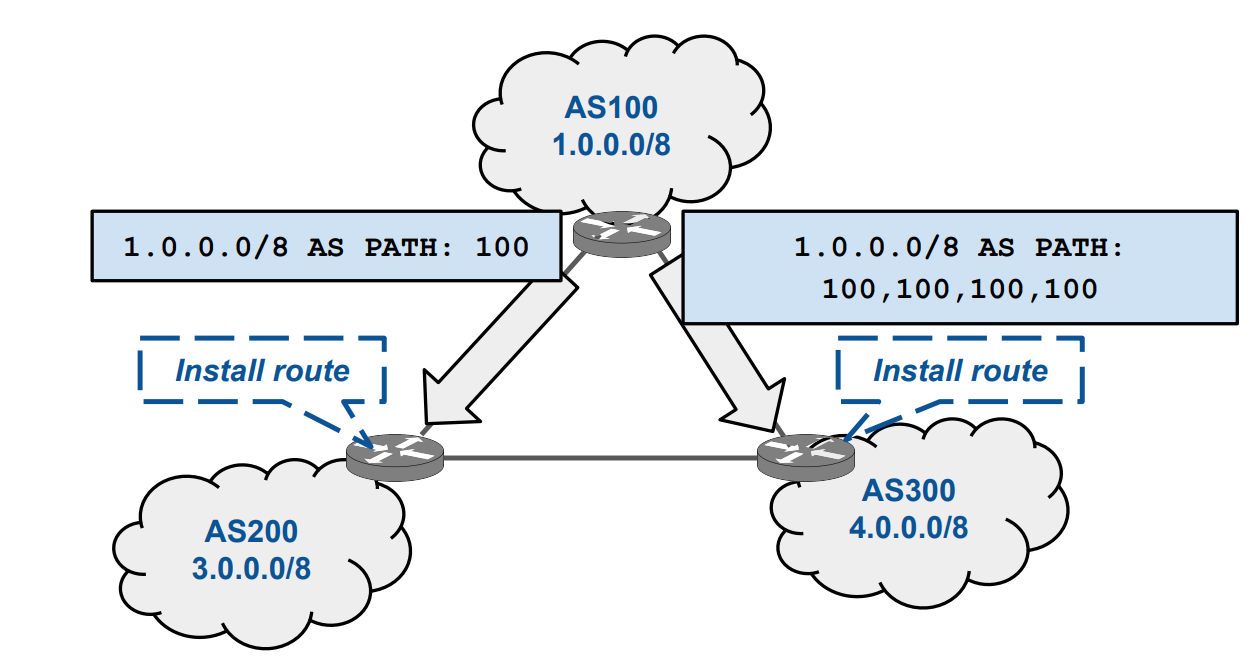
\includegraphics[width=0.75\textwidth]{immagini/NET_08/image_aspath_prepend.png}
\caption{Esempio di AS-PATH prepend per rendere meno appetibile un percorso verso 1.0.0.0/8.}
\end{figure}

\paragraph{Effetto sulla preferenza del percorso nei peer}

Negli esempi di AS-PATH prepend, a fronte di due annunci per lo stesso prefisso, un peer che vede:
\begin{itemize}
    \item un percorso con AS\_PATH “normale”;
    \item e un percorso alternativo con AS\_PATH contenente più ripetizioni dello stesso AS;
\end{itemize}
tende a preferire il primo, perché ha una lista di AS più corta. In questo modo è possibile orientare il traffico in ingresso facendo sì che alcuni peer “scartino” percorsi volutamente allungati e utilizzino link alternativi considerati più desiderabili.

\subsubsection{Community BGP}

\paragraph{Attributo COMMUNITY: struttura e uso operativo}

L’attributo \texttt{COMMUNITY} è un attributo \emph{optional transitive}: è un valore numerico associato a un prefisso e propagato ai neighbor. Quando un router riceve un annuncio con una certa community, può usare quel valore per applicare azioni predefinite, ad esempio filtrare la rotta o modificare altri attributi.

Una community BGP è un numero a 32 bit, rappresentabile come intero unico (0--4\,294\,967\,295) oppure come due interi a 16 bit separati da due punti (\texttt{0--65535:0--65535}), formato molto usato in pratica. Le community sono uno strumento essenziale per controllare topologie complesse, ad esempio nelle BGP/MPLS VPN.

\paragraph{Well-known communities: NO\_EXPORT, NO\_ADVERTISE, INTERNET, LOCAL-AS}

Le slide elencano alcune \emph{well-known standard communities}, che hanno significato condiviso:
\begin{itemize}
    \item \textbf{NO\_EXPORT}: la rotta non deve essere annunciata a peer esterni alla confederazione (o all’AS, se non sono usate confederazioni);
    \item \textbf{NO\_ADVERTISE}: la rotta non deve essere annunciata a \emph{nessun} peer BGP;
    \item \textbf{INTERNET}: la rotta può essere annunciata a tutti i peer, cioè resa visibile globalmente;
    \item \textbf{LOCAL-AS}: la rotta deve rimanere confinata all’interno dell’AS (o di un gruppo ristretto di peer interni) e non deve essere propagata a peer esterni.
\end{itemize}

Queste community permettono di controllare rapidamente la visibilità delle rotte senza dover definire regole complesse per ogni singolo neighbor.
\begin{figure}[H]
\centering
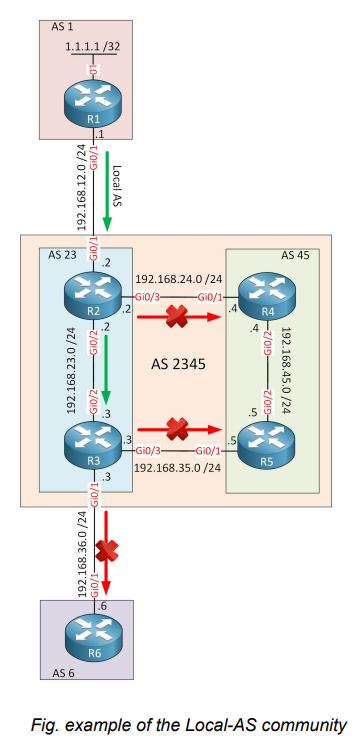
\includegraphics[width=0.35\textwidth]{immagini/NET_08/image_local_as_community.png}
\caption{Esempio operativo della community LOCAL-AS per limitare la propagazione di una rotta all’interno dell’AS.}
\end{figure}

\paragraph{Community personalizzate per politiche di routing e VPN}

Oltre alle well-known communities, le organizzazioni possono definire \emph{community personalizzate}. Le slide sottolineano che:
\begin{itemize}
    \item non esiste un unico schema globale: il significato delle community private è specifico a ciascun AS;
    \item non è necessario registrarle pubblicamente;
    \item possono codificare informazioni diverse (es. localizzazione geografica, tipo di servizio, livello di priorità, appartenenza a una certa VPN, ecc.).
\end{itemize}

In scenari avanzati, in particolare con BGP/MPLS VPN, queste community vengono usate per modellare topologie logiche (ad esempio quali siti devono essere interconnessi) e per applicare politiche di routing differenziate all’interno della stessa infrastruttura fisica.

\subsection{Configurazione di base di BGP (stile FRR/Cisco)}

\subsubsection{Definizione del processo BGP e annuncio delle reti}

\paragraph{Comando \texttt{router bgp <AS>} e significato del processo}

La configurazione di BGP in stile Cisco/FRR inizia con il comando:
\begin{center}
    \texttt{router bgp <AS-number>}
\end{center}
Questo comando abilita il processo BGP locale e associa il router a un determinato Autonomous System (AS). Tutti i comandi inseriti in questo contesto (\texttt{(config-router)}) configurano il comportamento del processo BGP per quell’AS. La sintassi ricorda quella degli IGP (come OSPF), ma il significato è diverso: non si attivano “istanze per interfaccia”, bensì un unico processo di frontiera verso altri router BGP appartenenti allo stesso AS (IBGP) o ad AS diversi (EBGP).

\paragraph{Comando \texttt{network} in BGP e differenze rispetto agli IGP}

Il comando:
\begin{center}
    \texttt{network <network-number> [mask <network-mask>]}
\end{center}
viene utilizzato per \emph{annunciare} reti tramite BGP. Negli IGP (es. OSPF) \texttt{network} serve a determinare su quali interfacce inviare e ricevere aggiornamenti; in BGP, invece, \texttt{network} \textbf{non} decide dove il protocollo gira, ma indica quali prefissi, già presenti nella routing table locale, devono essere inseriti negli UPDATE verso i neighbor. Le reti da annunciare possono essere directly connected, statiche o apprese tramite altri protocolli dinamici; se un prefisso non è presente nella tabella di routing, il comando \texttt{network} non ha effetto. L’opzione \texttt{mask} permette di specificare sottoreti puntuali.

\subsubsection{Configurazione dei neighbor}

\paragraph{Comando \texttt{neighbor <IP> remote-as <AS>}: peering EBGP e IBGP}

Il comando centrale per definire un peer BGP è:
\begin{center}
    \texttt{neighbor <ip-address> remote-as <AS-number>}
\end{center}
Esso identifica l’indirizzo IP del router remoto con cui instaurare una sessione BGP e specifica il suo AS di appartenenza. In base al valore di \texttt{remote-as}:
\begin{itemize}
    \item se l’AS remoto è diverso dall’AS locale, la sessione è di tipo \emph{EBGP};
    \item se l’AS remoto coincide con quello locale, si tratta di una sessione \emph{IBGP}.
\end{itemize}
Lo stesso comando viene usato sia su piattaforme Cisco sia in FRR, con semantica analoga.

\paragraph{Uso delle interfacce di loopback e concetto di BGP speaker}

Ogni router che esegue BGP è detto \emph{BGP speaker}. Le sessioni BGP possono utilizzare come indirizzo di peering sia indirizzi di interfacce fisiche sia indirizzi di interfacce di loopback. L’uso delle loopback è particolarmente indicato per i peer interni (IBGP), perché:
\begin{itemize}
    \item rende l’indirizzo del neighbor indipendente da una singola interfaccia fisica;
    \item mantiene la sessione stabile anche in presenza di più percorsi IP tra i router;
    \item si integra bene con un IGP che trasporta le route verso le loopback dei BGP speaker.
\end{itemize}
Una best practice comune è usare loopback per IBGP e interfacce fisiche per EBGP, salvo scenari di multilink.

\subsubsection{Loopback, update-source e robustezza}

\paragraph{Sessioni IBGP su loopback e multilink tra router interni}

Nel caso di IBGP, i router sono spesso collegati da più link interni e dispongono di connettività IP di livello 3 garantita da un IGP (ad esempio OSPF). Configurare il peering IBGP usando gli indirizzi di loopback dei router consente di sfruttare tutti i percorsi disponibili: finché l’IGP riesce a instradare verso la loopback del peer, la sessione BGP rimane attiva, indipendentemente dallo stato dei singoli link fisici. Questa tecnica è utile anche in caso di multilink, perché permette di bilanciare il traffico su più collegamenti sottostanti.

\paragraph{Comando \texttt{update-source loopback 0} e scelte del sorgente TCP}

Quando si utilizza una loopback per instaurare la sessione, è necessario indicare a BGP quale indirizzo di sorgente usare per la connessione TCP verso il neighbor. Il comando tipico è:
\begin{center}
    \texttt{neighbor <ip-address> update-source loopback 0}
\end{center}
che istruisce il router a usare l’indirizzo dell’interfaccia \texttt{Lo0} come indirizzo sorgente per la sessione BGP. Senza questo comando, il router userebbe di default l’indirizzo IP dell’interfaccia “più vicina” al peer, perdendo i vantaggi di robustezza forniti dalla loopback. Poiché le sessioni EBGP sono di solito point-to-point su un singolo link, l’uso di \texttt{update-source loopback 0} è tipicamente necessario solo per le sessioni IBGP.

\subsubsection{Gestione operativa del processo BGP}

\paragraph{Reset delle sessioni: \texttt{clear ip bgp *} e rischi in produzione}

Durante la configurazione o la modifica di BGP, i cambiamenti potrebbero non riflettersi immediatamente sulle sessioni esistenti. Per forzare un reset del processo BGP (con conseguente cancellazione della tabella BGP e riapertura delle sessioni) si può usare il comando:
\begin{center}
    \texttt{clear ip bgp *}
\end{center}
Questo comando interrompe e ristabilisce tutte le sessioni BGP del router, causando il ritiro temporaneo delle rotte e la successiva riconvergenza. In ambiente di produzione è fortemente raccomandato usare questo comando con estrema cautela, poiché può provocare disservizi estesi, come mostrato anche da casi reali di outage citati nelle slide.

\paragraph{Verifica con \texttt{show ip bgp} e \texttt{show ip bgp neighbors}}

Per verificare lo stato del processo BGP e delle rotte apprese, si utilizzano tipicamente:
\begin{itemize}
    \item \texttt{show ip bgp}: mostra la BGP table locale, il router ID, l’AS locale, i prefissi conosciuti e per ciascuno lo stato (\emph{valid}, \emph{best}), l’AS path, il next hop e altri attributi utili al troubleshooting;
    \item \texttt{show ip bgp neighbors}: mostra lo stato delle sessioni con ciascun neighbor (IBGP/EBGP), i parametri di negoziazione, i timer (hold time, keepalive), il conteggio di messaggi inviati/ricevuti e la durata della sessione.
\end{itemize}
Questi comandi sono lo strumento principale per controllare che le sessioni siano \emph{Established} e che le route BGP siano effettivamente presenti e coerenti con la configurazione.

\newpage
\maketitle
{\LARGE \textbf{Laboratorio}} \\[0.5em]
\subsection{Laboratorio: semplice scenario BGP con FRR}

\paragraph{Obiettivo.}
In questo laboratorio vengono esplorati i concetti di routing tra Autonomous Systems (AS) utilizzando BGP, con un focus sull'interconnessione di più AS tramite sessioni EBGP e la distribuzione delle rotte interne tramite IBGP. Viene inoltre testato come BGP interagisce con un IGP (OSPF) per garantire la connettività tra router all'interno di un singolo AS.

\paragraph{Topologia di rete.}
\begin{figure}[H]
\centering

\includegraphics[width=0.35\textwidth]{immagini/NET_08/topologia.png}
\end{figure}
L'ambiente di test comprende tre Autonomous Systems (AS100, AS200, AS300) e cinque router configurati come segue:
\begin{itemize}
    \item \textbf{AS100}: Router \textbf{R1}, che annuncia i prefissi \texttt{1.0.0.0/16} e \texttt{1.1.0.0/16}.
    \item \textbf{AS200}: Router \textbf{R2}, \textbf{R4}, e \textbf{R5}, che fungono da provider e gestiscono il routing tra AS100 e AS300.
    \item \textbf{AS300}: Router \textbf{R3}, che annuncia il prefisso \texttt{3.0.0.0/8}.
\end{itemize}
I collegamenti tra i router sono stabiliti tramite reti point-to-point:
\begin{itemize}
    \item R1-R2 con link \texttt{10.0.12.0/30};
    \item R2-R4-R5 con link \texttt{10.0.24.0/30}, \texttt{10.0.25.0/30}, e \texttt{10.0.45.0/30};
    \item R5-R3 con link \texttt{10.0.35.0/30}.
\end{itemize}

\paragraph{Separazione tra IGP e BGP.}
Nel laboratorio viene separato l’IGP interno (OSPF) da BGP, con OSPF che gestisce la connettività interna tra i router di AS200 e BGP che si occupa dell’interscambio di rotte tra AS. Questo approccio assicura che BGP possa sfruttare la connettività fornita da OSPF per stabilire le sessioni di peering IBGP (tra router dello stesso AS) e EBGP (tra AS diversi).

\subsubsection{Configurazione di routing interno (AS200)}

\paragraph{Indirizzamento IP e loopback per R2, R4, R5.}
Ogni router in AS200 è configurato con una loopback per identificare in modo univoco ogni dispositivo:
\begin{itemize}
    \item R2: \texttt{2.2.0.0/16} e \texttt{2.255.0.2/32};
    \item R4: \texttt{2.4.0.0/16} e \texttt{2.255.0.4/32};
    \item R5: \texttt{2.5.0.0/16} e \texttt{2.255.0.5/32}.
\end{itemize}
Le interfacce Ethernet (ad esempio \texttt{10.0.24.0/30}) connettono i router all’interno di AS200, consentendo la comunicazione tra R2, R4, e R5.

\paragraph{Configurazione OSPF in AS200.}
OSPF è configurato in area 0 per garantire la connettività interna:
\begin{itemize}
    \item Ogni router ha un \texttt{router-id} basato sull’indirizzo \texttt{2.255.0.x/32}.
    \item Le interfacce di transito e loopback sono incluse nelle configurazioni di OSPF con il comando \texttt{network}.
\end{itemize}

\subsubsection{Configurazione BGP nei diversi AS}

\paragraph{Annuncio dei prefissi locali.}
Ogni router annuncia i prefissi locali nel proprio AS utilizzando il comando \texttt{network}. Esempio:
\begin{itemize}
    \item \textbf{R1} (AS100): \texttt{router bgp 100}, \texttt{network 1.0.0.0/16}, \texttt{network 1.1.0.0/16};
    \item \textbf{R2, R4, R5} (AS200): \texttt{router bgp 200}, \texttt{network 2.2.0.0/16}, \texttt{network 2.4.0.0/16}, \texttt{network 2.5.0.0/16};
    \item \textbf{R3} (AS300): \texttt{router bgp 300}, \texttt{network 3.0.0.0/8}.
\end{itemize}

\paragraph{Peering EBGP.}
Le sessioni EBGP tra i confini degli AS sono configurate come segue:
\begin{itemize}
    \item Tra R1 (AS100) e R2 (AS200) su link \texttt{10.0.12.0/30};
    \item Tra R5 (AS200) e R3 (AS300) su link \texttt{10.0.35.0/30}.
\end{itemize}

\paragraph{Peering IBGP full-mesh in AS200.}
All’interno di AS200, R2, R4 e R5 sono configurati in modalità full-mesh per garantire che ogni router interno possa ricevere le rotte da ogni altro router:
\begin{itemize}
    \item R2 stabilisce sessioni IBGP con R4 e R5 utilizzando gli indirizzi loopback.
    \item R4 e R5 sono configurati in modo simile, utilizzando il comando \texttt{neighbor} con \texttt{update-source} e \texttt{next-hop-self}.
\end{itemize}

\subsubsection{Verifica e test di connettività}

\paragraph{Controlli con \texttt{show ip bgp summary}, \texttt{show ip bgp} e \texttt{show ip route}.}
Per verificare la corretta propagazione delle rotte, si utilizzano i seguenti comandi:
\begin{itemize}
    \item \texttt{show ip bgp summary}: verifica lo stato delle sessioni BGP (EBGP/IBGP).
    \item \texttt{show ip bgp}: mostra la BGP table e i prefissi appresi.
    \item \texttt{show ip route}: verifica la presenza dei prefissi BGP nella routing table globale.
\end{itemize}

\paragraph{Ping tra indirizzi di loopback in AS diversi.}
Per verificare la connettività end-to-end tra AS, si esegue un ping tra le loopback degli AS:
\begin{itemize}
    \item \texttt{ping 1.0.0.1 source 2.4.0.1} per R1 (AS100);
    \item \texttt{ping 3.0.0.1 source 2.4.0.1} per R3 (AS300).
\end{itemize}

I ping devono avere un tasso di successo del 100\%, confermando che il traffico è correttamente instradato tra gli AS.

\paragraph{Verifica della sessione BGP tramite `debug` (opzionale).}
Se le sessioni BGP non sono stabilite, è possibile eseguire il comando di debug per monitorare le comunicazioni BGP:
\begin{verbatim}
debug ip bgp
\end{verbatim}
Questo comando aiuta a diagnosticare problemi relativi alla connessione BGP e al flusso di aggiornamenti.

---

\paragraph{Conclusioni.}
Il laboratorio ha dimostrato come configurare un semplice scenario BGP con FRR tra diversi Autonomous Systems (AS), utilizzando sia EBGP che IBGP. È stata verificata la connettività tra gli AS e l'annuncio dei prefissi tra di essi. La configurazione ha anche incluso la gestione della routing table e dei comandi di monitoraggio.

---

\paragraph{Dettagli aggiuntivi:}
\begin{itemize}
    \item \textbf{Configurazione BGP:}
    \begin{itemize}
        \item È importante seguire l'ordine corretto nella configurazione di BGP su ogni router, stabilendo prima le sessioni EBGP e successivamente quelle IBGP.
        \item È necessario includere il comando \texttt{next-hop-self} nei peer IBGP per evitare problemi di instradamento.
    \end{itemize}

    \item \textbf{Test di Connettività:}
    \begin{itemize}
        \item Oltre ai ping, può essere utile fare un test di \textbf{traceroute} per verificare il percorso completo che i pacchetti seguono tra gli AS.
        \item Un altro test utile per verificare la propagazione delle rotte è eseguire un comando \texttt{show ip bgp} per ogni router e assicurarsi che le rotte siano correttamente propagate.
    \end{itemize}
\end{itemize}

\paragraph{Conclusioni.}
Con questa versione il laboratorio è completo e dettagliato, con tutte le informazioni necessarie per configurare, verificare e monitorare una rete BGP tra più Autonomous Systems.
